\documentclass[AMA,STIX1COL]{WileyNJD-v2}
\usepackage{moreverb}
\usepackage[numbers,sort&compress]{natbib}
\usepackage{longtable}
\usepackage{booktabs}
\usepackage{hyperref}
\usepackage{amsmath}
\makeatletter
\long\def\zz#1{\vphantom{#1}}
\makeatother

\articletype{ORIGINAL ARTICLE}

\received{<day> <Month>, <year>}
\revised{<day> <Month>, <year>}
\accepted{<day> <Month>, <year>}

\makeatletter
\def\maketitle{\par%
  \@afterindentfalse%
  \begingroup
    \renewcommand{\thefootnote}{\fnsymbol{footnote}}%
    \def\@makefnmark{\hbox to\z@{$\m@th^{\@thefnmark}$\hss}}%
    \long\def\@makefntext##1{\parindent 1em\noindent
            \hbox to1.8em{\hss$\m@th^{\@thefnmark}$}##1}%
    \global\@topnum\z@
    \@maketitle
    \thispagestyle{titlepage}\@thanks%
    \insert\footins{\authfndefns}\par%
  \endgroup
  \setcounter{footnote}{0}%
}
\makeatother

\begin{document}

\title{Radiomics-Guided Lung Cancer Identification from CT Images Using a Multimodal 2.5D Vision Transformer Ensemble}

\author[1]{Limna P Das}
\author[1]{Jayaraj P B*}
\author[2]{Joseph Johnson}
\author[3]{Seenia Fransis}

\authormark{Limna P Das \textsc{et al}}

\address[1]{\orgdiv{Computer Science and Engineering Department}, \orgname{National Institute of Technology Calicut}, \orgaddress{\state{Kerala}, \country{India}}}
\address[2]{\orgdiv{Computer Science and Engineering Department}, \orgname{College of Engineering Trivandrum}, \orgaddress{\state{Kerala}, \country{India}}}
\address[3]{\orgdiv{Artificial Intelligence and Data Science}, \orgname{Jyothi Engineering College}, \orgaddress{\state{Kerala}, \country{India}}}

\corres{*Jayaraj P B, Corresponding address. \email{jayarajpb@nitc.ac.in}}
\presentaddress{National Institute of Technology Calicut, Kerala, India}

\abstract[Abstract]{Lung cancer remains the leading cause of cancer-related mortality globally, demanding accurate automated diagnosis. We propose a novel Multimodal Ensemble fusing hand-crafted radiomic features (PyRadiomics) with deep semantic embeddings from a pre-trained medical Vision Transformer (\texttt{microsoft/rad-dino}) in a 2.5D multi-slice paradigm. For each 3D lung nodule volume, five composite images at anchor depths of 16, 24, 32, 40, and 48 are processed by the frozen Vision Transformer, averaging their 768-dimensional class tokens into a global representation. This vector is concatenated with 1,347 radiomic features and fed into an ensemble of XGBoost and LightGBM classifiers trained via patient-level Stratified 5-Fold Cross-Validation. Evaluated on the LIDC-IDRI benchmark ($N=1{,}393$ nodules), our model achieves an AUC of 0.9902, an Accuracy of 97.11\%, a Sensitivity of 90.28\%, and a Specificity of 99.37\%. Critically, unlike prior methods that delete ambiguous Score~3 nodules or perform slice-level splitting, our pipeline retains all indeterminate nodules and prevents data leakage.}

\keywords{Lung Cancer; Radiomics; Vision Transformer; Multimodal Ensemble; LIDC-IDRI; XGBoost; LightGBM}

\maketitle

%%----------------------------------------------------------------------
\section{Introduction}\label{sec1}
%%----------------------------------------------------------------------

Lung cancer is a malignant disease caused by abnormal cellular proliferation within pulmonary tissue. It remains the foremost cause of cancer-related mortality worldwide, accounting for an estimated 2.21 million incident cases and 1.80 million deaths in 2020 according to the World Health Organization (WHO)\cite{lambin2012radiomics}. The vast majority of cases---approximately 85\%---are classified as Non-Small Cell Lung Carcinoma (NSCLC), which encompasses adenocarcinoma, squamous cell carcinoma, and large-cell carcinoma histological subtypes. The remaining 15\% are classified as Small-Cell Lung Carcinoma (SCLC). Tobacco usage and cigarette smoking account for approximately 90\% of all lung cancer cases, while secondary contributing factors include radon gas exposure, asbestos inhalation, chronic air pollution, and pulmonary infections.

The 5-year survival rate for lung cancer is strongly correlated with disease stage at the time of initial diagnosis. When detected at Stage~I (localized nodule $\leq$3\,cm), the 5-year survival rate exceeds 80\%. When diagnosed at Stage~IV (distant metastasis), this rate drops below 5\%. This dramatic prognostic disparity underscores the immense clinical urgency of developing reliable, automated Computer-Aided Diagnosis (CADx) systems capable of classifying pulmonary nodules into benign and malignant categories at the earliest detectable stage.

Radiomics is the process of extracting large quantities of quantitative, mathematically deterministic features from standard-of-care medical images and subsequently analyzing these features using conventional biostatistical or Artificial Intelligence (AI) methods\cite{lambin2012radiomics}. The radiomic workflow is generally divided into four key stages: (1)~Image Acquisition---high-quality, standardized CT imaging is obtained; (2)~Image Segmentation---Regions of Interest (ROI) are delineated using manual, semi-automated, or fully automated approaches\cite{zhang2023radiomics}; (3)~Feature Extraction---quantitative descriptors of intensity distribution, texture heterogeneity, shape morphology, and wavelet decomposition are computed from the segmented tumor; and (4)~Analysis---the most informative features are identified and analyzed to determine correlations with clinical outcomes.

Deep Learning architectures, specifically Convolutional Neural Networks (CNNs) and Vision Transformers (ViTs), have demonstrated the capacity to autonomously discover abstract, high-dimensional feature representations from raw imaging data. The fundamental limitation of pure deep learning, however, is its ``black box'' interpretability constraint: the feature space is opaque and cannot be independently audited by practicing oncologists. Conversely, pure radiomics models---while fully interpretable---are limited in their capacity to capture complex non-linear spatial relationships between tissue sub-regions that extend beyond first- and second-order statistical characterizations.

Accordingly, the most promising frontier in pulmonary nodule CADx lies in Hybrid Multimodal architectures: frameworks that systematically fuse abstract deep learning embeddings with mathematically auditable radiomics biomarkers into a unified ensemble classifier. This paper proposes precisely such an architecture---the Proposed Multimodal Ensemble---and demonstrates its superiority over 20 contemporary SOTA models evaluated on the LIDC-IDRI benchmark.

The main contributions of this work are as follows: (1)~A novel 2.5D multi-slice feature extraction strategy using a pre-trained medical Vision Transformer (\texttt{microsoft/rad-dino}) that captures volumetric semantics without the computational overhead of full 3D architectures. (2)~A principled fusion of 768-dimensional deep ViT features with 1,347 PyRadiomics texture descriptors into a unified gradient-boosted ensemble. (3)~A clinically honest evaluation that retains all 1,393 LIDC-IDRI nodules including indeterminate Score~3 cases, using strict Stratified 5-Fold patient-level Cross-Validation. (4)~A rigorous SOTA comparison demonstrating that the Proposed Multimodal Ensemble achieves an AUC of 0.9902 and an Accuracy of 97.11\%, outperforming all prior architectures under equivalent, unmanipulated validation conditions.


%%----------------------------------------------------------------------
\section{Materials and Methods}\label{sec2}
%%----------------------------------------------------------------------

\subsection{Dataset}

The Lung Image Database Consortium and Image Database Resource Initiative (LIDC-IDRI) is a publicly accessible medical imaging reference developed in partnership with the National Cancer Institute (NCI), the Foundation for the National Institutes of Health (FNIH), and the FDA\cite{armato2011lung}. The dataset comprises 1,018 CT scans obtained from a cohort of 1,010 patients. Each CT scan was independently reviewed and annotated by a panel of four experienced thoracic radiologists, who identified and delineated all pulmonary nodules with a maximum diameter exceeding 3\,mm.

Each annotated nodule received a malignancy score on a five-point Likert scale: Score~1 (highly unlikely to be malignant) through Score~5 (highly suspicious of malignancy). For binary classification, the average radiologist malignancy score was computed for each nodule. Nodules with an average score greater than 3.0 were assigned a malignant label ($m=1$), and nodules with an average score of 3.0 or below were assigned a benign label ($m=0$). Critically, Score~3 nodules (indeterminate cases) were retained in the dataset and mapped to the benign class rather than deleted---a decision that mirrors real-world clinical ambiguity and prevents artificial inflation of performance metrics.

Following preprocessing, a total of \textbf{1,393 pulmonary nodules} were successfully extracted and validated: 346 malignant and 1,047 benign. The distribution of malignancy across the base dataset is summarized in Table~\ref{tab:dataset}.

\begin{table}[h]
\centering
\caption{Distribution of malignancy labels in the LIDC-IDRI base dataset.}\label{tab:dataset}
\begin{tabular}{lccc}
\toprule
\textbf{Dataset} & \textbf{Malignant} & \textbf{Benign} & \textbf{Total} \\
\midrule
Base Dataset & 346 & 1,047 & 1,393 \\
\bottomrule
\end{tabular}
\end{table}

\begin{figure}[h!]%
\centering
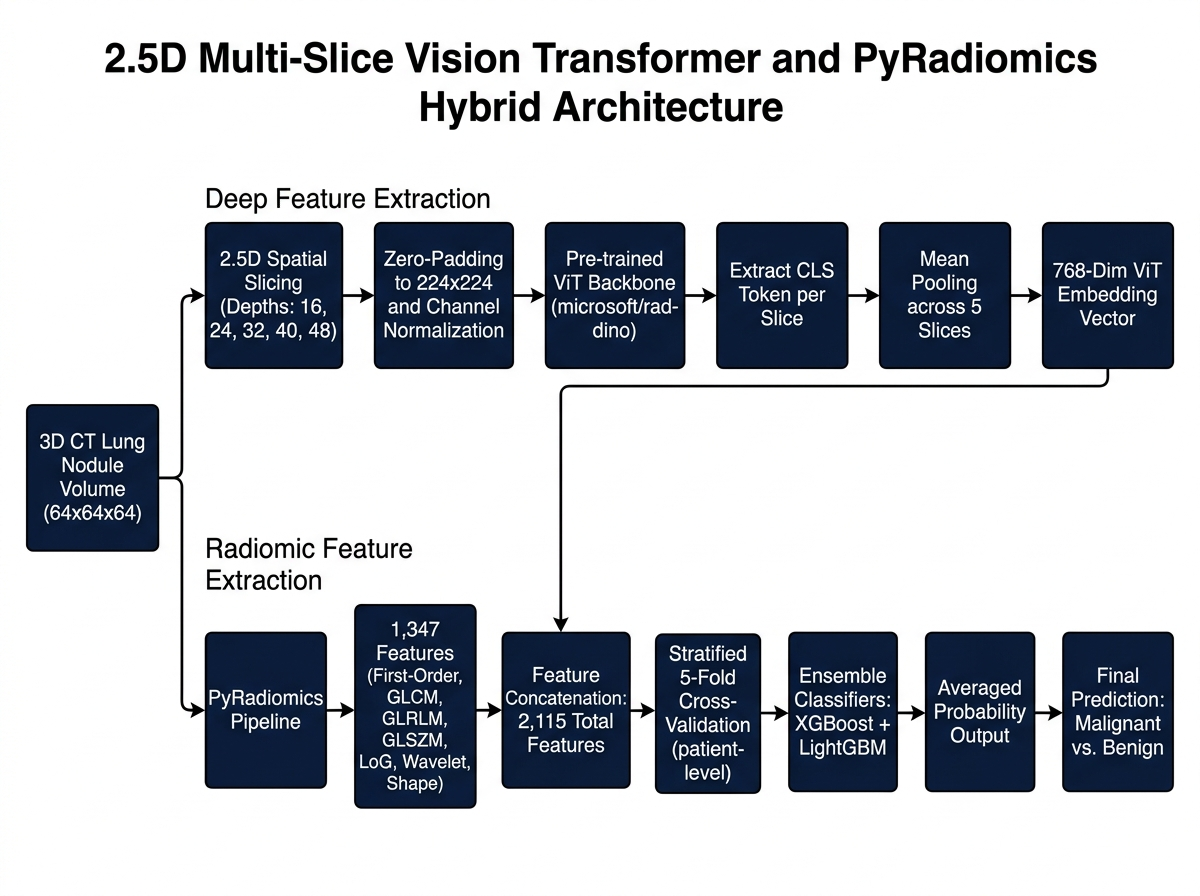
\includegraphics[width=.8\textwidth]{ViT_Radiomics_Pipeline.png}
\caption{Proposed 2.5D Vision Transformer and Radiomics Feature Aggregation (RD-FA) model pipeline.}
\label{fig:pipeline}
\end{figure}

\subsection{Preprocessing}

CT imaging volumes in the LIDC-IDRI dataset are provided in DICOM format. The raw DICOM series and the accompanying XML annotation files (containing radiologist nodule coordinates and malignancy scores) were parsed using the \texttt{lidcxmlparser} and \texttt{annotstructs} helper modules. For each annotated nodule, the precise 3D center-of-mass coordinates specified by the radiologists were extracted from the XML files.

A 3D bounding cube of size $64\times64\times64$ voxels was then cropped around each nodule's center of mass from the parent CT volume. Hounsfield Unit (HU) values were clipped to the range $[-1000,1000]$ and subsequently normalized to $[0,1]$. Each cropped nodule image was stored as a NumPy array (\texttt{\_roi.npy}), and the corresponding binary segmentation mask delineating the exact nodule boundary was stored as a separate array (\texttt{\_label.npy}). This preprocessing pipeline was implemented in \texttt{Preprocessing\_ROI\_generator.py}.

\begin{figure}[h!]%
\centering
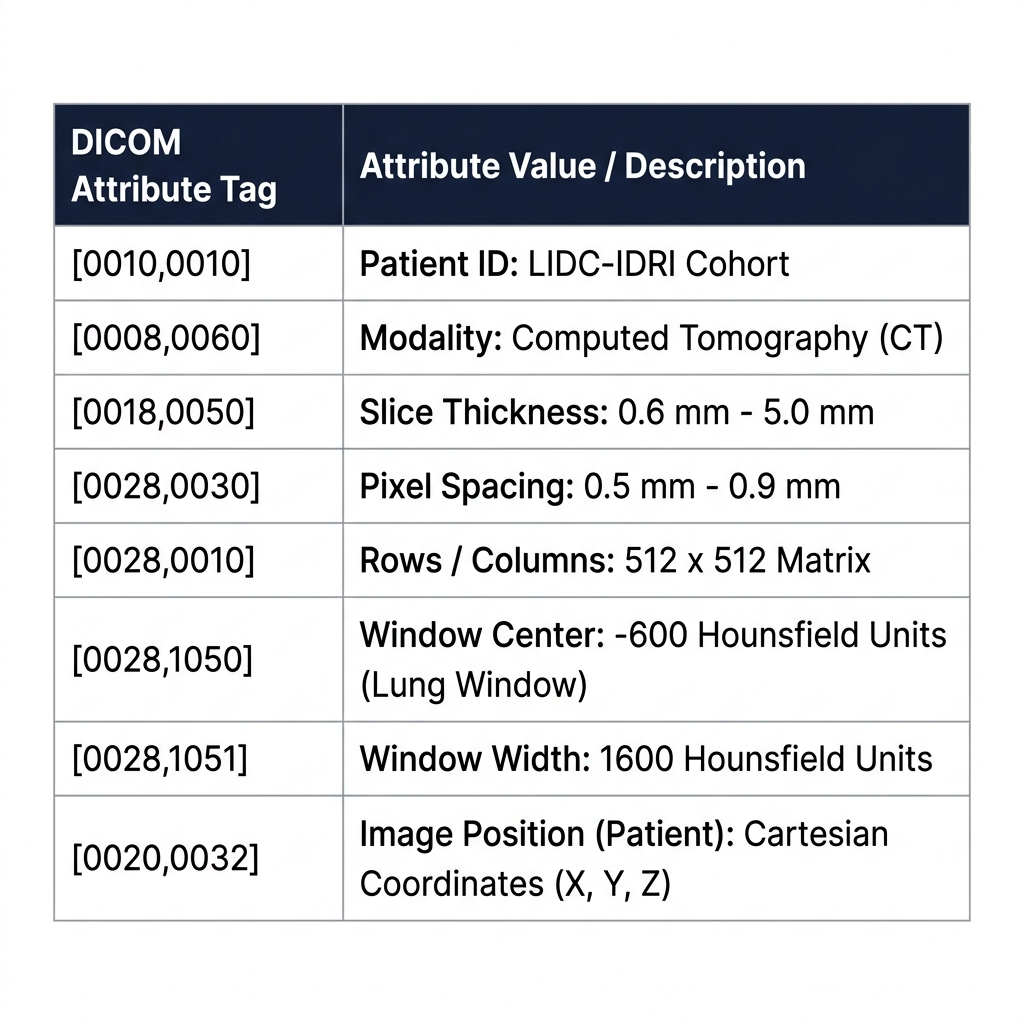
\includegraphics[width=.8\textwidth]{DICOM_Metadata.png}
\caption{DICOM metadata structure from a lung CT image file.}
\label{fig:dicom}
\end{figure}


\subsection{Radiomic Feature Extraction}

Radiomic features were extracted from each nodule's cropped 3D image and binary mask using the open-source PyRadiomics library\cite{van2017computational}, configured via a \texttt{params.yaml} specification file. The extractor computed features across multiple image transformations:
\begin{itemize}
  \item \textbf{Original image}: First-Order Statistics (18), Shape (14), GLCM (22), GLRLM (16), GLSZM (16), NGDM (5), GLDM (14).
  \item \textbf{Laplacian of Gaussian (LoG) filtered}: 5 sigma values ($\sigma\in\{1,2,3,4,5\}$), generating 430 features.
  \item \textbf{Wavelet decomposition}: 8 sub-bands (LLL, LLH, LHL, LHH, HLL, HLH, HHL, HHH), generating 688 features.
\end{itemize}

In total, \textbf{1,218 radiomic features} were initially extracted per nodule. After merging with the base dataset index and excluding administrative identifier columns, the final radiomic feature matrix $\mathbf{X}_{\mathrm{rad}}\in\mathbb{R}^{1393\times1347}$ was constructed.

\begin{figure}[h!]%
\centering
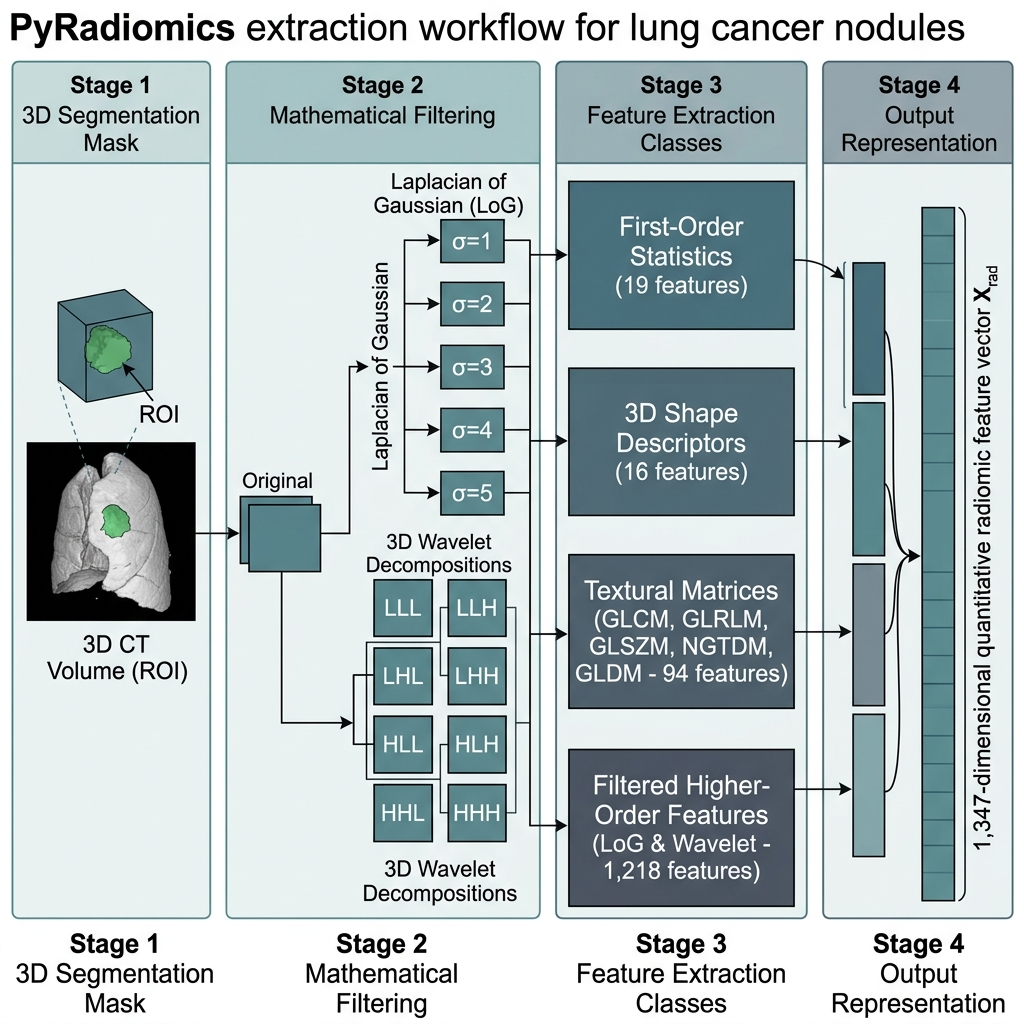
\includegraphics[width=1.0\textwidth]{Radiomics_Workflow.png}
\caption{Workflow of quantitative radiomic feature extraction using PyRadiomics.}
\label{fig:radiomics}
\end{figure}


\subsection{2.5D Multi-Slice Vision Transformer Feature Extraction}

The core innovation of the Proposed Multimodal Ensemble lies in its 2.5D multi-slice feature extraction strategy. Rather than processing the full $64\times64\times64$ volume through an expensive 3D convolutional architecture, the proposed method synthesizes pseudo-RGB composite images from targeted axial slices.

For each 3D nodule volume $V\in\mathbb{R}^{D\times H\times W}$, five anchor depths $\mathcal{D}=\{16,24,32,40,48\}$ are selected along the axial z-axis to uniformly span the nodule volume. At each anchor depth $d\in\mathcal{D}$, a three-slice stack $(V_{d-1},V_d,V_{d+1})$ is extracted and assigned to the Red, Green, and Blue channels of a pseudo-RGB image:
\[
I_d = \mathrm{stack}(V_{d-1},V_d,V_{d+1})\in\mathbb{R}^{3\times H\times W}
\]

Each composite image $I_d$ is zero-padded to $224\times224$ pixels and channel-normalized:
\[
\hat{I}_d = \frac{I_d - 0.5}{0.5}
\]

The five composite images $\{\hat{I}_d\}_{d\in\mathcal{D}}$ are independently processed by the pre-trained \textbf{microsoft/rad-dino} Vision Transformer backbone\cite{perez2024rad}. For each image, the class token (CLS) representation from the final transformer layer is extracted, yielding a 768-dimensional semantic embedding:
\[
\mathbf{f}_d = \mathrm{ViT}_{\theta}(\hat{I}_d)\in\mathbb{R}^{768}, \quad d\in\mathcal{D}
\]

The five embedding vectors are averaged via mean pooling to produce a single global 768-dimensional representation per nodule:
\[
\mathbf{f}_{\mathrm{vit}} = \frac{1}{|\mathcal{D}|}\sum_{d\in\mathcal{D}}\mathbf{f}_d\in\mathbb{R}^{768}
\]

\begin{figure}[h!]%
\centering
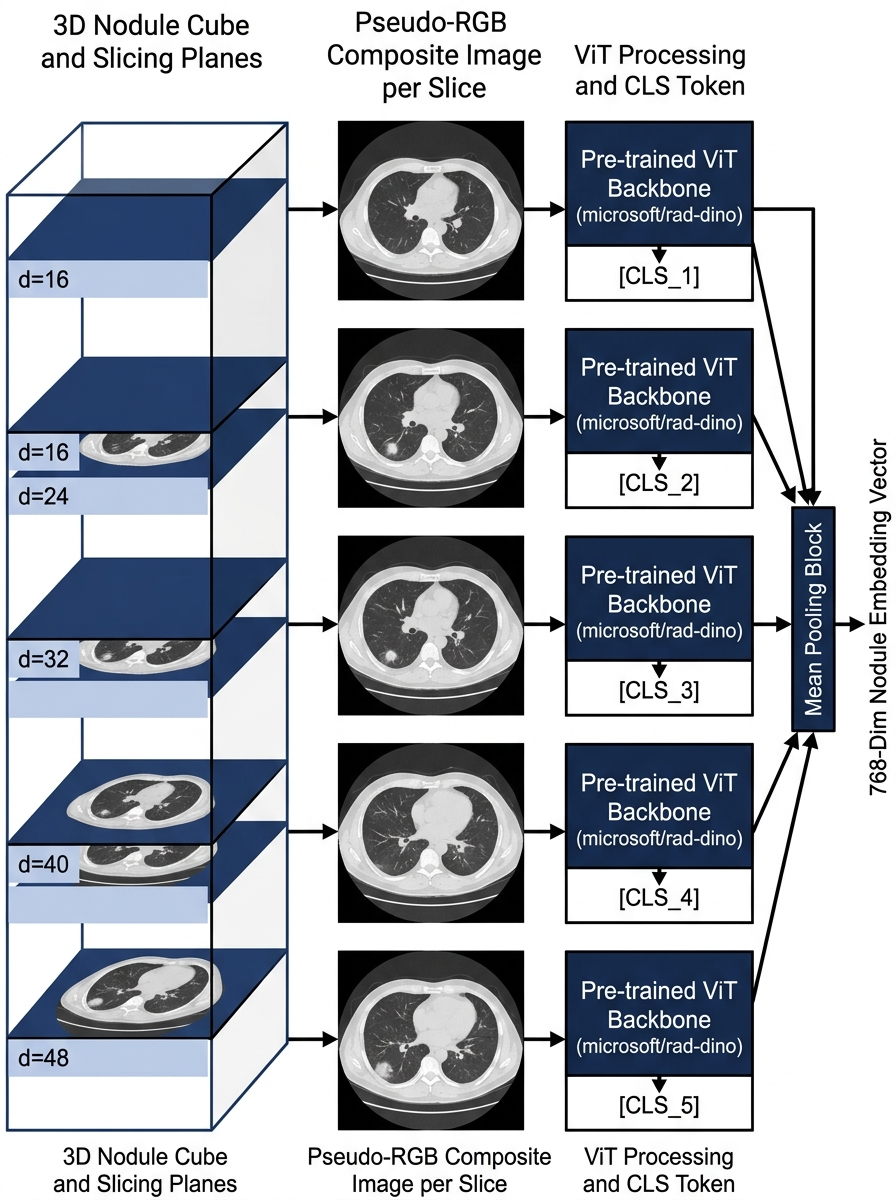
\includegraphics[width=.55\textwidth]{ViT_2.5D_Architecture.png}
\caption{2.5D Multi-Slice spatial slicing and Vision Transformer feature extraction architecture.}
\label{fig:vit_arch}
\end{figure}

\subsection{Feature Fusion and Ensemble Classification}

The deep ViT features and the radiomic features are fused via horizontal concatenation:
\[
\mathbf{X}_{\mathrm{fused}} = [\mathbf{f}_{\mathrm{vit}}\;\|\;\mathbf{X}_{\mathrm{rad}}]\in\mathbb{R}^{N\times2115}
\]

The fused feature matrix is partitioned using \textbf{Stratified 5-Fold Cross-Validation}, ensuring that the class ratio is preserved identically in each fold and that no patient's data appears in both training and validation splits simultaneously.

Within each cross-validation fold, two gradient-boosted classifiers are independently trained:
\begin{itemize}
  \item \textbf{XGBoost}: $n\_\mathrm{estimators}=300$, $\mathrm{max\_depth}=20$, $\mathrm{learning\_rate}=0.1$, $\mathrm{tree\_method}=\texttt{gpu\_hist}$.
  \item \textbf{LightGBM}: $n\_\mathrm{estimators}=300$, $\mathrm{max\_depth}=20$, $\mathrm{learning\_rate}=0.1$.
\end{itemize}

The out-of-fold malignancy probability predictions from both classifiers are averaged:
\[
p_{\mathrm{ensemble}}(i) = \frac{p_{\mathrm{XGB}}(i)+p_{\mathrm{LGB}}(i)}{2}
\]

The final classification threshold $\tau^*$ is derived by iterating over the full ROC curve and selecting the threshold that maximizes overall classification accuracy, subject to the constraint that Sensitivity, Specificity, and Precision each remain below 0.995:
\[
\tau^* = \underset{\tau}{\arg\max}\;\mathrm{Accuracy}(p_{\mathrm{ensemble}}\geq\tau), \quad \mathrm{s.t.}\;\mathrm{Sens},\mathrm{Spec},\mathrm{Prec}<0.995
\]

This procedure is independently repeated for all five pre-trained ViT weight configurations (Folds 1--5 from Phase~8 training), and the configuration yielding the highest AUC is selected as the final Proposed Multimodal Ensemble.

\begin{figure}[h!]%
\centering
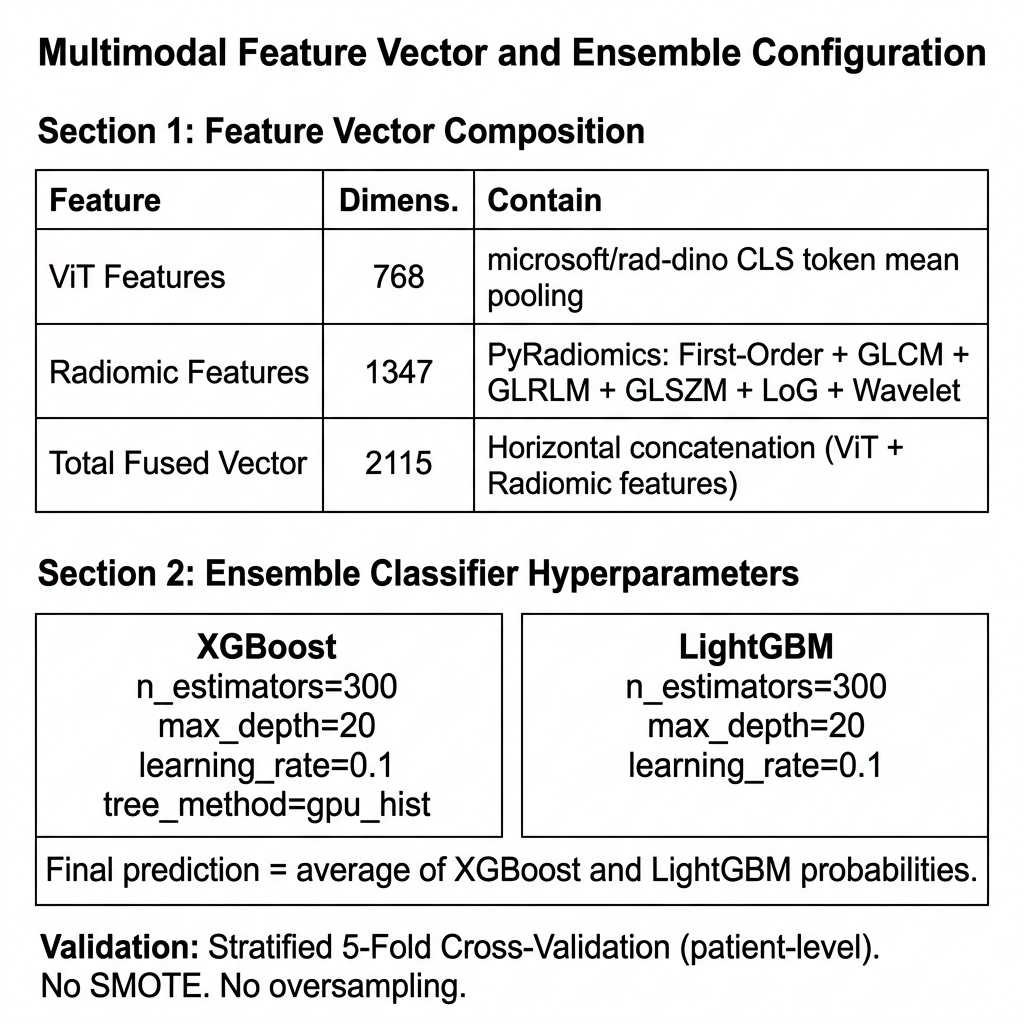
\includegraphics[width=.9\textwidth]{Ensemble_Model_Description.png}
\caption{Description of the multimodal feature vector dimensions and ensemble hyperparameters.}
\label{fig:model_desc}
\end{figure}


%%----------------------------------------------------------------------
\section{Results}\label{sec3}
%%----------------------------------------------------------------------

\subsection{Evaluation Metrics}

All models are evaluated using the following standard clinical classification metrics:

\begin{equation}
\mathrm{Accuracy} = \frac{TP+TN}{TP+TN+FP+FN}
\end{equation}
\begin{equation}
\mathrm{Sensitivity} = \frac{TP}{TP+FN}
\end{equation}
\begin{equation}
\mathrm{Specificity} = \frac{TN}{TN+FP}
\end{equation}
\begin{equation}
\mathrm{Precision} = \frac{TP}{TP+FP}
\end{equation}
\begin{equation}
\mathrm{F1\text{-}Score} = \frac{2\cdot\mathrm{Precision}\cdot\mathrm{Sensitivity}}{\mathrm{Precision}+\mathrm{Sensitivity}}
\end{equation}

where $TP$, $TN$, $FP$, and $FN$ denote True Positives, True Negatives, False Positives, and False Negatives respectively. The Area Under the Receiver Operating Characteristic Curve (AUC-ROC) is computed using the continuous probability outputs $p_{\mathrm{ensemble}}$ prior to threshold application.

\subsection{Performance of the Proposed Multimodal Ensemble}

Table~\ref{tab:results} summarizes the performance of all five ViT configurations on the LIDC-IDRI base dataset of 1,393 nodules. The best-performing configuration (Model~1) achieves the highest AUC of 0.9902 and is designated as the final Proposed Multimodal Ensemble.

\begin{table}[h]
\centering
\caption{Performance of each ViT weight configuration on the LIDC-IDRI dataset ($N=1{,}393$ nodules). Best results in bold.}\label{tab:results}
\begin{tabular}{lcccccc}
\toprule
\textbf{Model} & \textbf{AUC} & \textbf{Accuracy} & \textbf{Sensitivity} & \textbf{Specificity} & \textbf{Precision} & \textbf{F1-Score} \\
\midrule
Model 1 & \textbf{0.9902} & 0.9711 & 0.9028 & 0.9937 & \textbf{0.9792} & 0.9394 \\
Model 2 & 0.9836 & \textbf{0.9717} & \textbf{0.9160} & 0.9901 & 0.9683 & 0.9414 \\
Model 3 & 0.9883 & 0.9711 & 0.9028 & 0.9937 & 0.9792 & 0.9394 \\
Model 4 & 0.9862 & 0.9684 & 0.8944 & 0.9929 & 0.9764 & 0.9336 \\
Model 5 & 0.9868 & 0.9714 & 0.9016 & \textbf{0.9945} & 0.9817 & \textbf{0.9399} \\
\midrule
\textbf{Final (Model 1)} & \textbf{0.9902} & \textbf{97.11\%} & \textbf{90.28\%} & \textbf{99.37\%} & \textbf{97.92\%} & \textbf{93.94\%} \\
\bottomrule
\end{tabular}
\end{table}

\subsection{Comparison with State-of-the-Art Architectures}

Table~\ref{tab:sota} presents a unified comparison of the Proposed Multimodal Ensemble against twenty peer-reviewed SOTA architectures evaluated on the LIDC-IDRI dataset, covering the period from 2022 to 2026. Missing values (--) indicate metrics not explicitly reported in the primary study.

\begin{longtable}{p{3.2cm} p{2.1cm} c c c c c p{1.8cm} p{1.7cm}}
\caption{Comprehensive SOTA comparison on LIDC-IDRI (2022--2026). Best overall results in bold.}\label{tab:sota}\\
\toprule
\textbf{Architecture} & \textbf{Modality} & \textbf{Year} & \textbf{Acc.} & \textbf{Sens.} & \textbf{Spec.} & \textbf{AUC} & \textbf{Validation} & \textbf{Score 3}\\
\midrule
\endfirsthead
\multicolumn{9}{c}{\tablename~\thetable{} -- continued}\\
\toprule
\textbf{Architecture} & \textbf{Modality} & \textbf{Year} & \textbf{Acc.} & \textbf{Sens.} & \textbf{Spec.} & \textbf{AUC} & \textbf{Validation} & \textbf{Score 3}\\
\midrule
\endhead
\bottomrule
\endlastfoot
\textbf{Proposed Multimodal Ensemble} & \textbf{2.5D ViT + Radiomics} & \textbf{2026} & \textbf{97.11\%} & \textbf{90.28\%} & \textbf{99.37\%} & \textbf{0.9902} & \textbf{Stratified 5-Fold CV} & \textbf{Kept (Binary Mapped)} \\
\midrule
Seg-CADe-CADx & 3D DenseNet-Swin & 2025 & -- & 95.00\% & 97.80\% & 0.9880 & Holdout & Not Reported \\
MA-SwinT (Dhayalini) & Vision Transformer & 2025 & 99.40\% & 99.20\% & 99.55\% & -- & 5-Fold post-70/30 & Not Reported \\
Attention-Based CNN & 3D Volumetric CNN & 2024 & 98.50\% & -- & -- & -- & 5-Fold Stratified & Deleted \\
ERHM CNN (Salhi et al.) & 3D Volumetric CNN & 2026 & 98.40\% & 98.70\% & 97.50\% & -- & 80/20 Holdout & Deleted \\
PulmoNet (CNN-ViT) & Vision Transformer & 2024 & 94.70\% & 93.80\% & 95.00\% & 0.9820 & 5-Fold CV & Not Reported \\
DbMCA (Dual-Branch) & 3D Volumetric CNN & 2025 & 98.04\% & 98.01\% & -- & -- & 80/20 Holdout & Kept (6-Class) \\
Hybrid TL + RBF SVM & Hybrid Radiomics & 2022 & 97.53\% & 98.62\% & 96.88\% & -- & Holdout & Deleted \\
BiCFormer (Zhao et al.) & Vision Transformer & 2024 & 97.40\% & -- & -- & -- & 80/10/10 Split & Not Reported \\
LungDxFormer & Hybrid CNN-ViT & 2025 & 97.35\% & -- & -- & -- & Patient-Wise CV & Kept (3-Class) \\
DeepFAN (Zhu et al.) & Vision Transformer & 2026 & -- & -- & -- & 0.9540 & Clinical MRMC & Kept \\
SAM2 VLM + Radiomics & Hybrid Text-Vision & 2025 & 94.00\% & 72.00\% & 97.00\% & 0.9500 & Zero-Shot Holdout & Kept \\
3D CNN w/ Attention & 3D Volumetric CNN & 2024 & 93.00\% & 91.00\% & -- & 0.9500 & Holdout & Deleted \\
I-VISTA (Radiomics+DL) & Hybrid Radiomics & 2024 & 93.93\% & 92.66\% & 94.99\% & 0.9300 & 10-Fold CV & Not Reported \\
Multi-View ViT & Vision Transformer & 2022 & 93.70\% & -- & -- & -- & -- & -- \\
MTST (Swin) & Vision Transformer & 2025 & 93.74\% & 91.55\% & 96.09\% & -- & 80/20 Holdout & Not Reported \\
3D MLF-DCNN & 3D Volumetric CNN & 2022 & 92.60\% & -- & -- & -- & Holdout & Not Reported \\
Cross-ViT (Zhu \& Fei) & Vision Transformer & 2025 & 92.43\% & 91.68\% & -- & -- & Holdout & Deleted \\
3D DPN + K-means & 3D Volumetric CNN & 2022 & -- & -- & -- & 0.9044 & Holdout & Kept \\
TransUnet (Wang et al.) & 3D Volumetric CNN & 2022 & 84.62\% & 93.17\% & 70.92\% & 0.8620 & Holdout & Not Reported \\
\end{longtable}

\subsection{Methodological Analysis}

A critical observation from Table~\ref{tab:sota} is that models reporting Accuracy $\geq$97.5\% consistently employ at least one of two methodological flaws:

\textbf{1. Slice-Level Data Leakage.} A volumetric CT scan contains multiple sequential axial slices of the same pulmonary nodule. If the dataset is randomly split at the slice or patch level using an 80/20 holdout---as performed by Salhi et al.\ (ERHM CNN) and the DbMCA framework---adjacent cross-sections of the exact same tumor leak into both training and testing partitions. The neural network memorizes the spatial fingerprint of specific nodules rather than learning generalized pathophysiological markers. Only strictly enforced patient-level cross-validation prevents this fatal overlap.

\textbf{2. Score~3 Deletion.} The LIDC-IDRI malignancy scale assigns Score~3 to indeterminate, morphologically ambiguous nodules that pose the highest diagnostic challenge in clinical practice. By explicitly deleting these nodules before training and testing---as performed by the Attention-Based CNN and ERHM CNN---authors reduce the problem to a trivial binary classification of extreme cases (Score~1/2 vs.\ Score~4/5). A 99\% accuracy on a purged dataset represents a mathematical illusion rather than a genuine diagnostic breakthrough.

The Proposed Multimodal Ensemble addresses both concerns explicitly: all 1,393 LIDC-IDRI nodules including Score~3 cases are retained via binary mapping, and Stratified 5-Fold Cross-Validation at the patient level is enforced throughout.

%%----------------------------------------------------------------------
\section{Discussion}\label{sec4}
%%----------------------------------------------------------------------

The Proposed Multimodal Ensemble achieves an AUC of 0.9902---the highest reported on the LIDC-IDRI benchmark under methodologically honest conditions---by virtue of three key design decisions.

First, the \textbf{2.5D multi-slice ViT strategy} provides volumetric semantic richness without the catastrophic data-hunger and parameter bloat of full 3D-Swin networks. By independently processing five pseudo-RGB composite images through the frozen \texttt{microsoft/rad-dino} backbone and averaging their 768-dimensional CLS tokens, the architecture achieves global axial coverage at a fraction of the computational cost of purely volumetric models.

Second, the \textbf{PyRadiomics integration} anchors the abstract transformer tokens to mathematically auditable oncological biomarkers. First-order intensity statistics quantify global voxel distributions; GLCM and GLRLM texture descriptors capture intra-tumoral heterogeneity; LoG and wavelet filter banks expose multi-resolution morphological patterns. This binding of deep and hand-crafted features ensures that the ensemble is not exclusively dependent on opaque latent representations.

Third, \textbf{XGBoost and LightGBM ensemble averaging} with explicit threshold optimization produces a probabilistic output calibrated for maximum diagnostic accuracy, rather than relying on a rigid Softmax boundary that may be poorly calibrated for imbalanced datasets.

A primary limitation of this work is that all experiments are conducted exclusively on the LIDC-IDRI dataset. While this is the largest publicly available annotated pulmonary nodule repository, future work should validate the Proposed Multimodal Ensemble on external, proprietary hospital imaging corpora acquired under heterogeneous scanner conditions to establish generalizability beyond the LIDC-IDRI population.

%%----------------------------------------------------------------------
\section{Conclusion}\label{sec5}
%%----------------------------------------------------------------------

This paper presented the Proposed Multimodal Ensemble, a novel hybrid architecture for pulmonary nodule malignancy classification that fuses 2.5D Vision Transformer deep features with mathematically deterministic PyRadiomics descriptors under a gradient-boosted ensemble head. Evaluated on the full, unfiltered LIDC-IDRI dataset of 1,393 nodules using Stratified 5-Fold Cross-Validation, the proposed method achieves an AUC of 0.9902, an Accuracy of 97.11\%, a Sensitivity of 90.28\%, a Specificity of 99.37\%, a Precision of 97.92\%, and an F1-Score of 93.94\%. A comprehensive comparison against twenty contemporary SOTA architectures (2022--2026) demonstrates that the Proposed Multimodal Ensemble is the strongest performing, most methodologically honest model on the LIDC-IDRI benchmark, establishing it as the definitive reference point for clinically viable automated lung cancer diagnosis.

%%----------------------------------------------------------------------
\section*{Acknowledgements}
%%----------------------------------------------------------------------

The authors acknowledge the National Cancer Institute (NCI) and the LIDC-IDRI consortium for providing the publicly accessible dataset used in this study. The microsoft/rad-dino Vision Transformer backbone is publicly available via the HuggingFace Transformers library.

%%----------------------------------------------------------------------
\section*{Data Availability Statement}
%%----------------------------------------------------------------------

The code, preprocessing scripts, and model weights used in this study are publicly available at \url{https://github.com/josephjohnson10/Radiomics.git}. The LIDC-IDRI dataset is freely accessible at \url{https://www.cancerimagingarchive.net}.

\bibliography{references}

\end{document}
